\documentclass[a4paper,t,xcolor=pst,dvips,colortheme]{beamer}

\usepackage{beamerthemesplit}
\usepackage[utf8]{inputenc}
\usepackage[spanish]{babel}
\usepackage{graphicx}
\usepackage{pstricks} % PSTricks package
\usepackage{setspace}
\usepackage{multirow}
\usepackage{listings}
\usepackage{pgfpages}
\usepackage{hyperref}
\usepackage{etoolbox}
\usepackage{epstopdf}

\makeatletter
\patchcmd{\beamer@sectionintoc}{\vskip1.5em}{\vskip0.5em}{}{}
\makeatother

\setbeamercovered{dynamic}
\setcounter{tocdepth}{2}
\setbeamercolor{frametitle}{fg=black,bg=white}
\setbeamercolor{section in toc shaded}{fg=black}
\setbeamercolor{section in toc}{fg=red}
\setbeamercolor{subsection in toc shaded}{fg=black}
\setbeamercolor{subsection in toc}{fg=red}
\setbeamerfont{section in toc}{size=\small}
\setbeamerfont{subsection in toc}{size=\small}
\setbeamertemplate{section in toc shaded}[default][99]
\setbeamertemplate{subsection in toc shaded}[default][99]

\AtBeginSection[]
{\begin{frame}[c]
  \frametitle{Índice}
	\tableofcontents[currentsection,
        sectionstyle=show/shaded,
        subsectionstyle=hide]
\end{frame}}

\AtBeginSubsection[]
{\begin{frame}[c]
	\frametitle{Índice}
	\tableofcontents[
  		currentsection,
  		sectionstyle=shaded/shaded,
  		currentsubsection,
  		subsectionstyle=show/shaded/hide
		]
\end{frame}}

\setbeamercolor{frametitle}{fg=black,bg=white}

\setbeamertemplate{frametitle}{
	\begin{centering}
		\insertframetitle
		\par
	\end{centering}
}

\usetheme[secheader]{Boadilla} 

\title[Introducción a las Arq. Empresariales]{Introducción a las Arquitecturas Empresariales}

\author[Pablo Sánchez]{\alert{Pablo Sánchez}}

\institute[IIE]{
		   Dpto. Ingeniería Informática y Electrónica \\
		   Universidad de Cantabria \\
		   Santander (Cantabria, España) \\
		   \texttt{p.sanchez@unican.es}
}

\date{}

\begin{document}

\begin{frame}[c]
	\titlepage
	\begin{columns}
		\column{0.50\linewidth}
			\centering
    		
\includegraphics[width=.28\textwidth,keepaspectratio=true]{images/istr.eps}
		\column{0.50\linewidth}
			\centering
			
\includegraphics[width=.25\textwidth,keepaspectratio=true]{images/uc.eps}
	\end{columns}
\end{frame}

\begin{frame}[c]
    \frametitle{\alert{Advertencia}}
    \begin{center}
        Todo el material contenido en este documento no constituye en modo alguno una obra de referencia o apuntes oficiales mediante el cual se puedan preparar las pruebas evaluables necesarias para superar la asignatura. \ \\
        \ \\
        Este documento contiene exclusivamente una serie de diapositivas cuyo objetivo es servir de complemento visual a las actividades realizadas en el aula para la transmisión del contenido sobre el cual versarán las mencionadas pruebas evaluables.  \ \\
        \ \\
        Dicho de forma más clara, \alert{estas transparencias no son apuntes y su objetivo no es servir para que el alumno pueda preparar la asignatura.}
    \end{center}
\end{frame}

\section{Introducción}

\begin{frame}[c]
    \frametitle{Objetivos del Tema}
    \begin{enumerate}[<+->]
         \item Comprender qué es un \emph{Sistema de Información Empresarial}.
         \item Comprender el concepto de \emph{Arquitectura Software}.
         \item Conocer los principales patrones arquitectónicos que aplican a los Sistemas de Información Empresarial.
         \item Comprender cómo se divide un sistema empresarial en capas.
         \item Comprender la función de cada capa de un sistema sw.
         \item Conocer las tecnologías que se utilizan para implementar las capas de un sistema sw.
         \item Comprender cómo se pueden independizar módulos sw mediante \emph{inyección de dependencias}.
    \end{enumerate}
\end{frame}

\begin{frame}[c]
    \frametitle{Bibliografía}
    \begin{thebibliography}{1}

        \bibitem[Fowler, 2002]{Fowler2002x}
        Fowler, M. (2002).
        \newblock {\em {Patterns of Enterprise Application Architecture}}.
        \newblock Addison-Wesley Professional.

        \bibitem[Esposito and Saltarello, 2014]{Esposito2014x}
        Esposito, D. and Saltarello, A. (2014).
        \newblock {\em {Microsoft .NET - Architecting Applications for the
          Enterprise}}.
        \newblock 2 edition.

        \bibitem[Taylor et~al., 2009]{taylor:2009x}
        Taylor, R.~N., Medvidovic, N., and Dashofy, E. (2009).
        \newblock {\em {Software Architecture: Foundations, Theory, and Practice}}.
        \newblock Wiley.

    \end{thebibliography}
\end{frame}

\section{Sistemas de Información Empresarial}

\begin{frame}
    \frametitle{Sistema de Información Empresarial}
    \begin{block}{Sistema Empresarial}
        Sistema sw que da soporte a diferentes procesos de negocio de una determinada organización.
    \end{block}
    \uncover<2->{
    \begin{block}{Características de los Sistemas de Información Empresariales}
    \begin{enumerate}
        \item<3-> Necesita almacenar datos, y normalmente, en gran volumen.
        \item<4-> Los datos que almacenan representan un activo importante y duradero en el tiempo.
        \item<5-> Se accede de forma concurrente a los datos. Se precisan \emph{transacciones}.
        \item<6-> Requieren múltiples y avanzados sistemas de presentación y navegación de datos.
        \item<7-> Interoperan con otros sistemas empresariales.
        \item<8-> Los manipulación de los datos debe obedecer a ciertas reglas.
    \end{enumerate}
    \end{block}
    }
\end{frame}

\section{Arquitecturas Sw}

\subsection{Concepto de Arquitectura Sw}

\begin{frame}[t]
   \frametitle{Fases del Ciclo de Vida Sw}
   \only<1|handout:0>{
	   \rput[lt](0.5,-0.5){
	   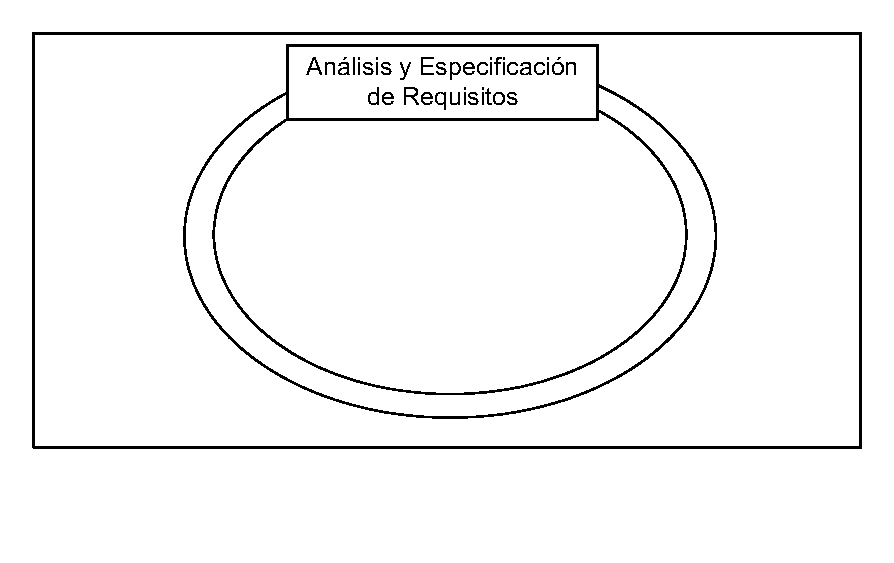
\includegraphics[width=11cm,keepaspectratio=true]{images/ciclosVida/ciclo00.eps}}
   }
   \only<2|handout:1>{
	   \rput[lt](0.5,-0.5){
	   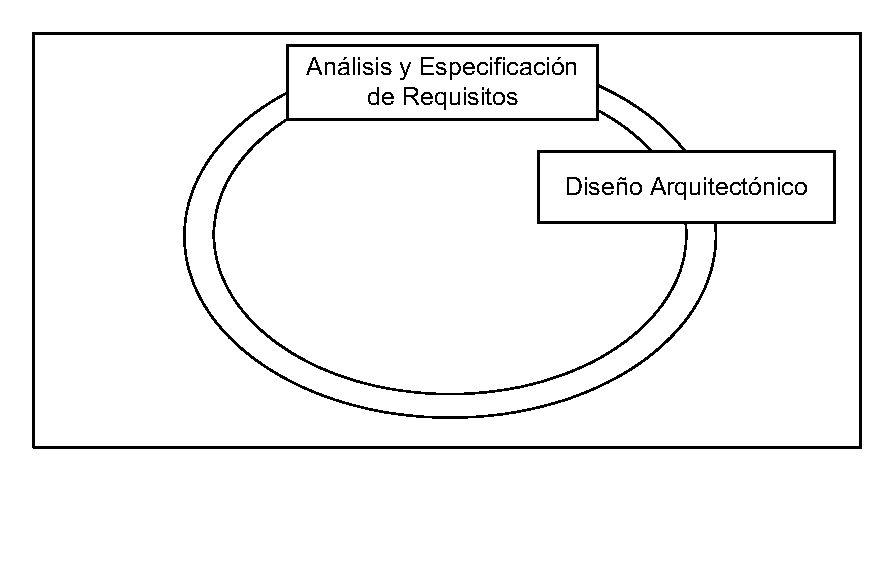
\includegraphics[width=11cm,keepaspectratio=true]{images/ciclosVida/ciclo01.eps}}
   }
\end{frame}

\begin{frame}[t]
	\frametitle{¿Por Qué Necesitamos Arquitecturas Sw?}
    \only<1|handout:0>{
	   \rput[lt](0.5,0.25){
        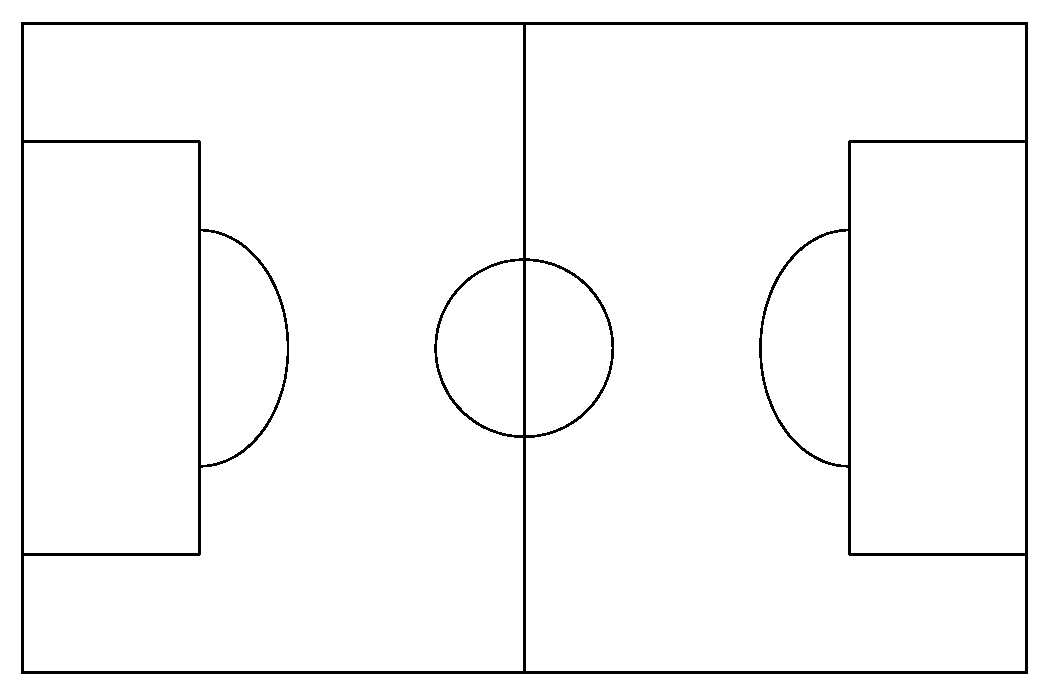
\includegraphics[width=11cm,keepaspectratio=true]{images/introduccion/futbol00.eps}}
	}
	\only<2|handout:0>{
	   \rput[lt](0.5,0.25){
	   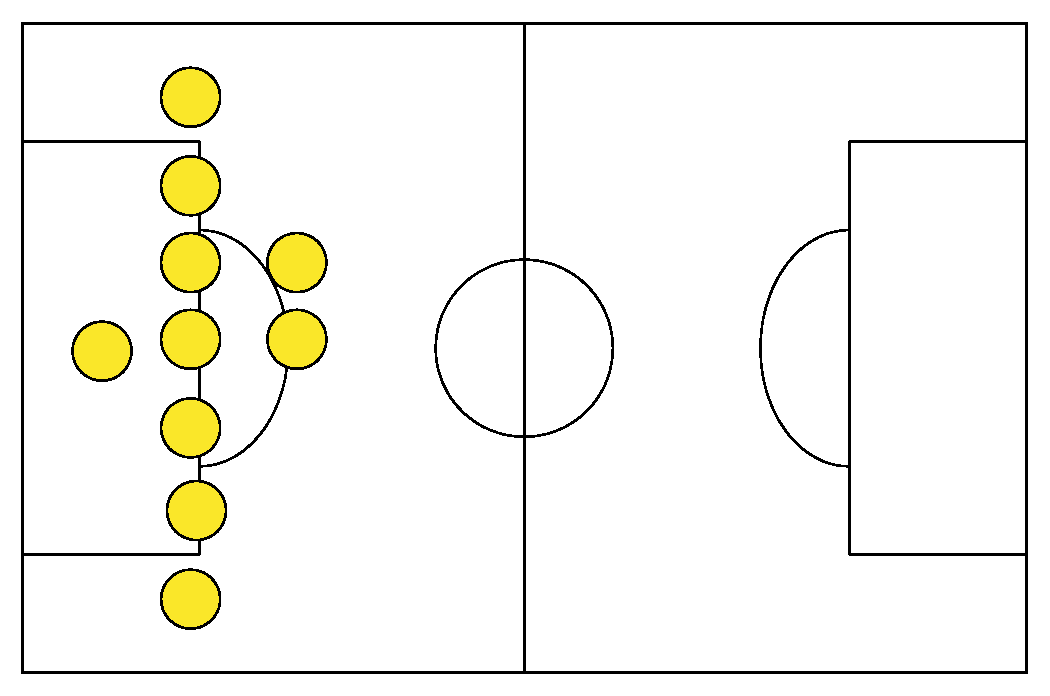
\includegraphics[width=11cm,keepaspectratio=true]{images/introduccion/futbol01.eps}}
	}
	\only<3|handout:0>{
	   \rput[lt](0.5,0.25){
	   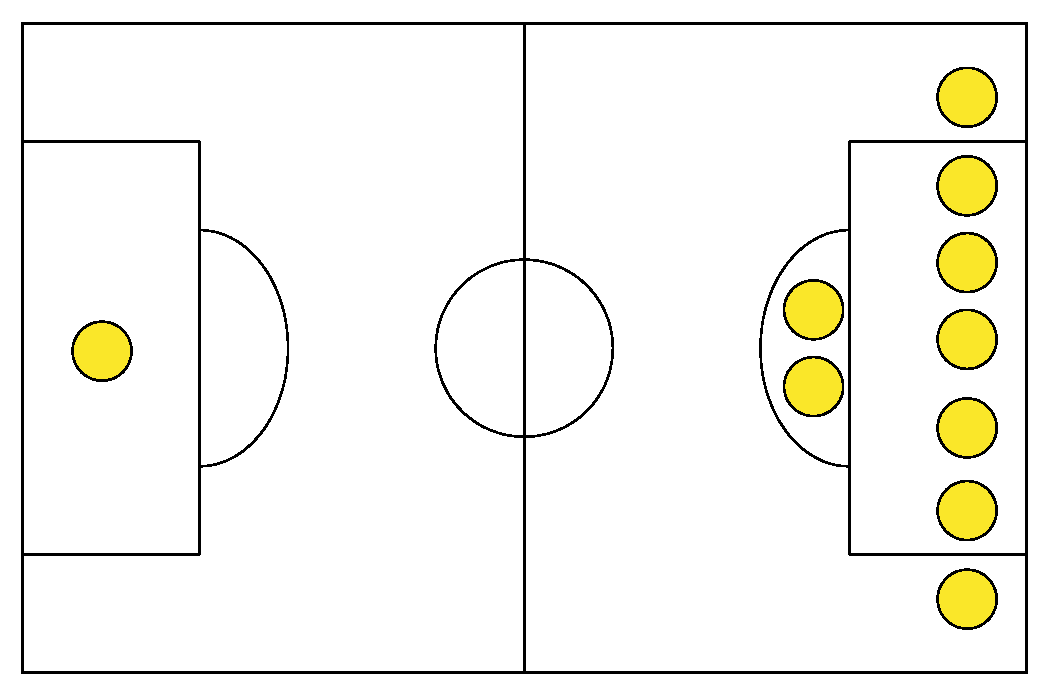
\includegraphics[width=11cm,keepaspectratio=true]{images/introduccion/futbol02.eps}}
	}
	\only<4|handout:1>{
	   \rput[lt](0.5,0.25){
	   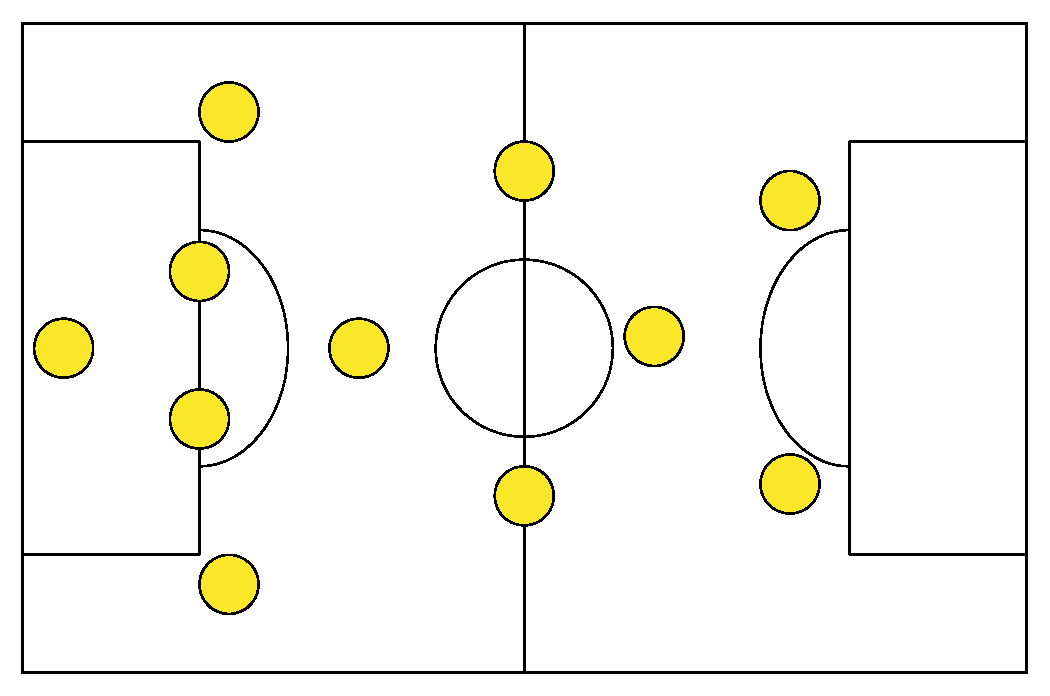
\includegraphics[width=11cm,keepaspectratio=true]{images/introduccion/futbol03.eps}}
	}
	\only<5|handout:0>{
	   \rput[lt](0.5,0.25){
	   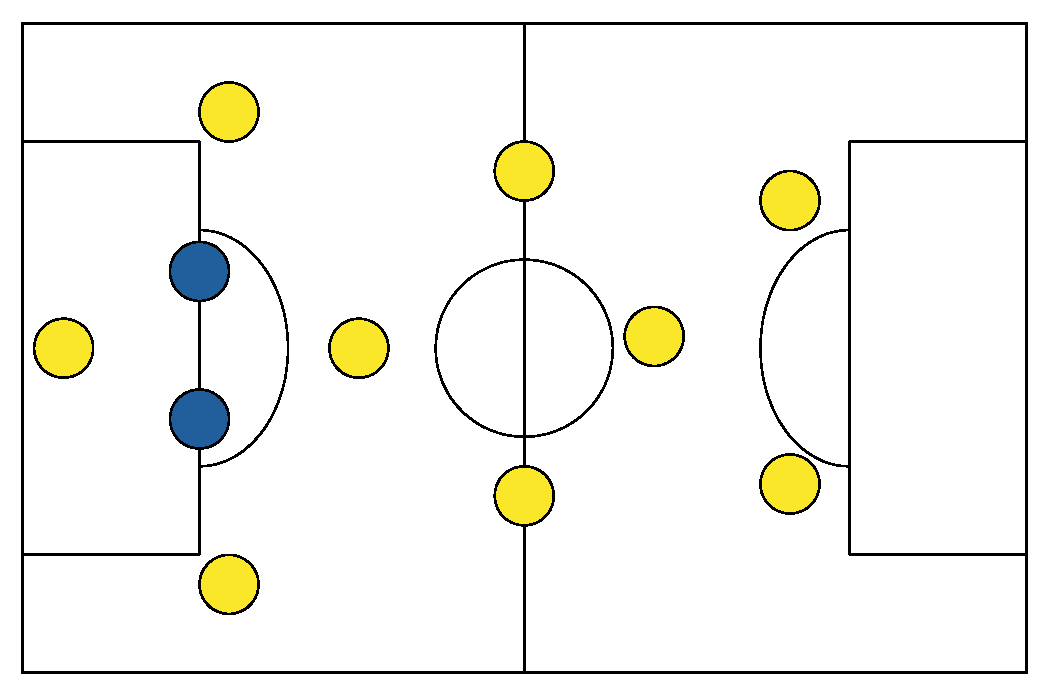
\includegraphics[width=11cm,keepaspectratio=true]{images/introduccion/futbol04.eps}}
	}
	\only<6|handout:0>{
	   \rput[lt](0.5,0.25){
	   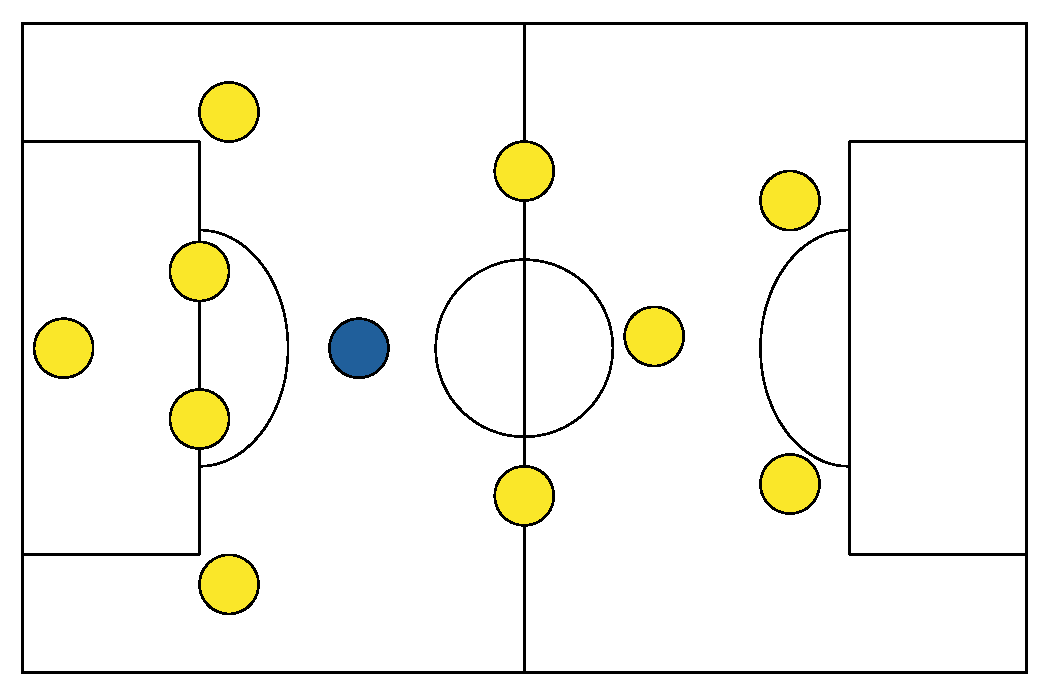
\includegraphics[width=11cm,keepaspectratio=true]{images/introduccion/futbol05.eps}}
	}
	\only<7|handout:0>{
	   \rput[lt](0.5,0.25){
	   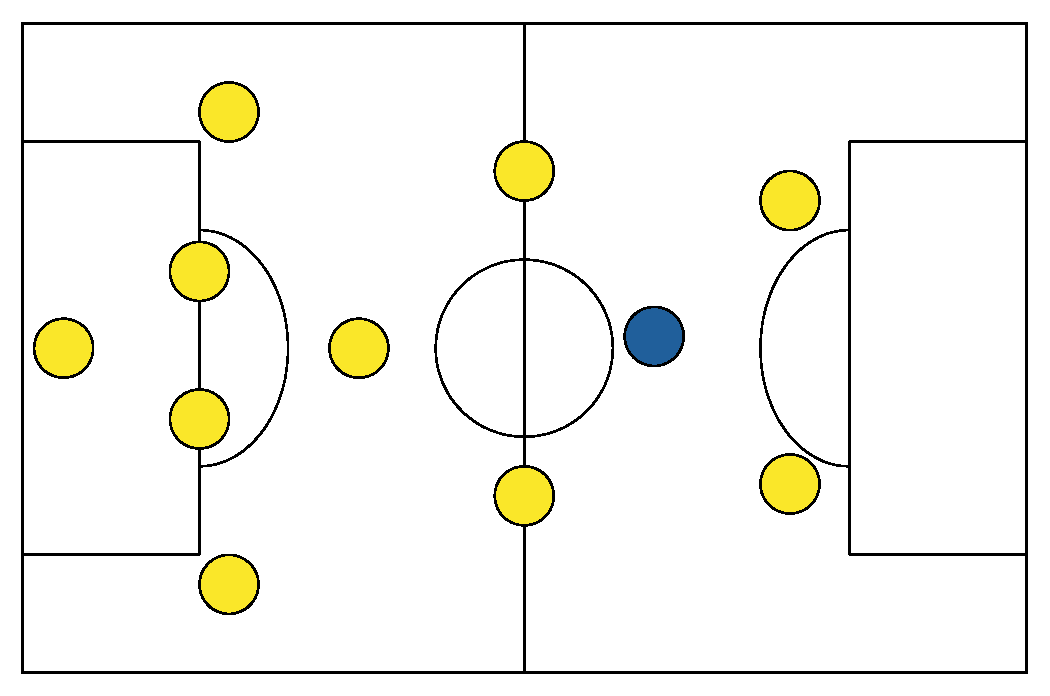
\includegraphics[width=11cm,keepaspectratio=true]{images/introduccion/futbol06.eps}}
	}
	\only<8|handout:0>{
	   \rput[lt](0.5,0.25){
	   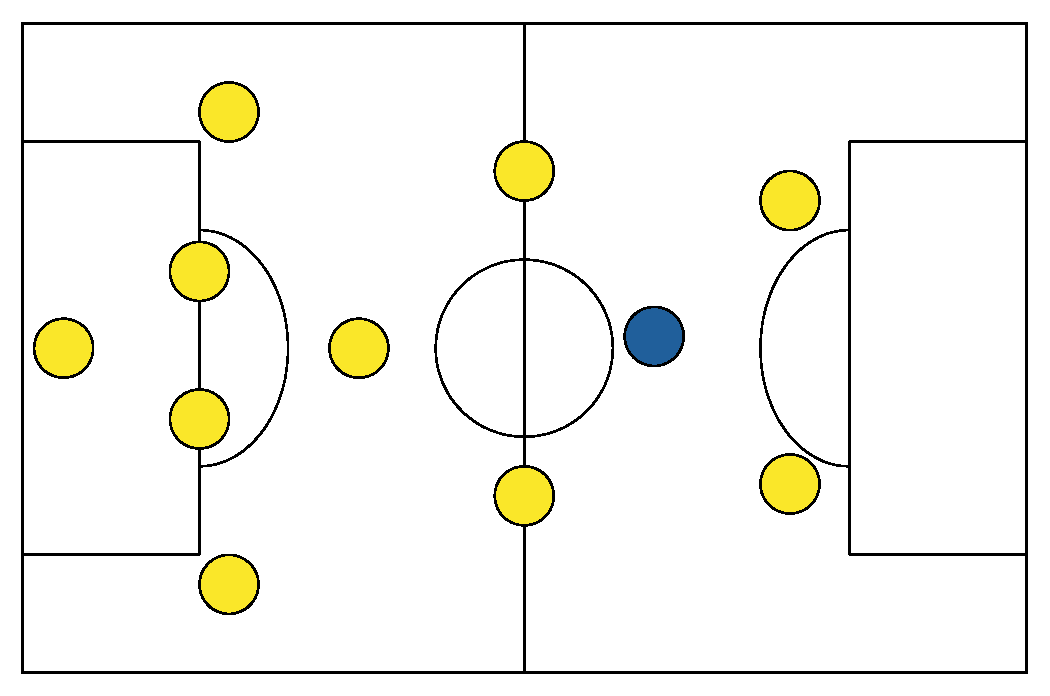
\includegraphics[width=11cm,keepaspectratio=true]{images/introduccion/futbol06.eps}}
	}
\end{frame}

\subsection{Definición de Arquitectura Sw}

\begin{frame}[t]
	\frametitle{Definiciones Arquitectura Sw}
	\begin{block}{Arquitectura Software~\cite{taylor:2009,pohl:2005}}
		La arquitectura de un sistema sw es el conjunto de las principales decisiones de diseñoo realizadas sobre el sistema. Toda arquitectura sw tiene una \emph{estructura} y una \emph{textura}.
	\end{block}
	\uncover<2->{
		\begin{block}{Textura Arquitectónica~\cite{jazayeri:2000,pohl:2005}}
			La \emph{textura} de un arquitectura sw es el conjunto de reglas que gobiernan el desarrollo y diseño de un sistema software.
		\end{block}
	}
	\uncover<3->{
		\begin{block}{Estructura Arquitectónica~\cite{jazayeri:2000,pohl:2005}}
			La \emph{estructura} de una arquitectura sw es la descomposición de un sistema sw en sus partes principales y las relaciones entre dichas partes.
		\end{block}
	}
\end{frame}

\subsection{Patrones Arquitectónicos}

\begin{frame}[c]
	\frametitle{Patrones Arquitectónicos}
    \begin{block}{Patrón Arquitectónico}
        Un \emph{patrón arquitectónico} es un conjunto con nombre de decisiones de diseño reutilizables Y aplicables a problemas de diseño arquitectónico recurrentes, pero que necesitan ser adaptadas a cada sistema concreto.
	\end{block}
\end{frame}

\subsubsection{Arquitecturas en Capas}

\begin{frame}[c]
    \frametitle{Arquitecturas en Capas - Principio Básico}
    \begin{block}{Arquitecturas en Capas}
        \begin{itemize}[<+->]
            \item Un sistema se descompone en un conjunto de capas.
            \item Las capas se diseñan de abajo a arriba.
            \item Cada capa manipula un conjunto bien definido de elementos, ofreciendo un \alert{conjunto potente y estable de abstracciones} para la manipulación de dichos elementos a las capas superiores.
        \end{itemize}
    \end{block}
\end{frame}

\begin{frame}[c]
	\frametitle{Arquitecturas en Capas}
	\begin{center}
        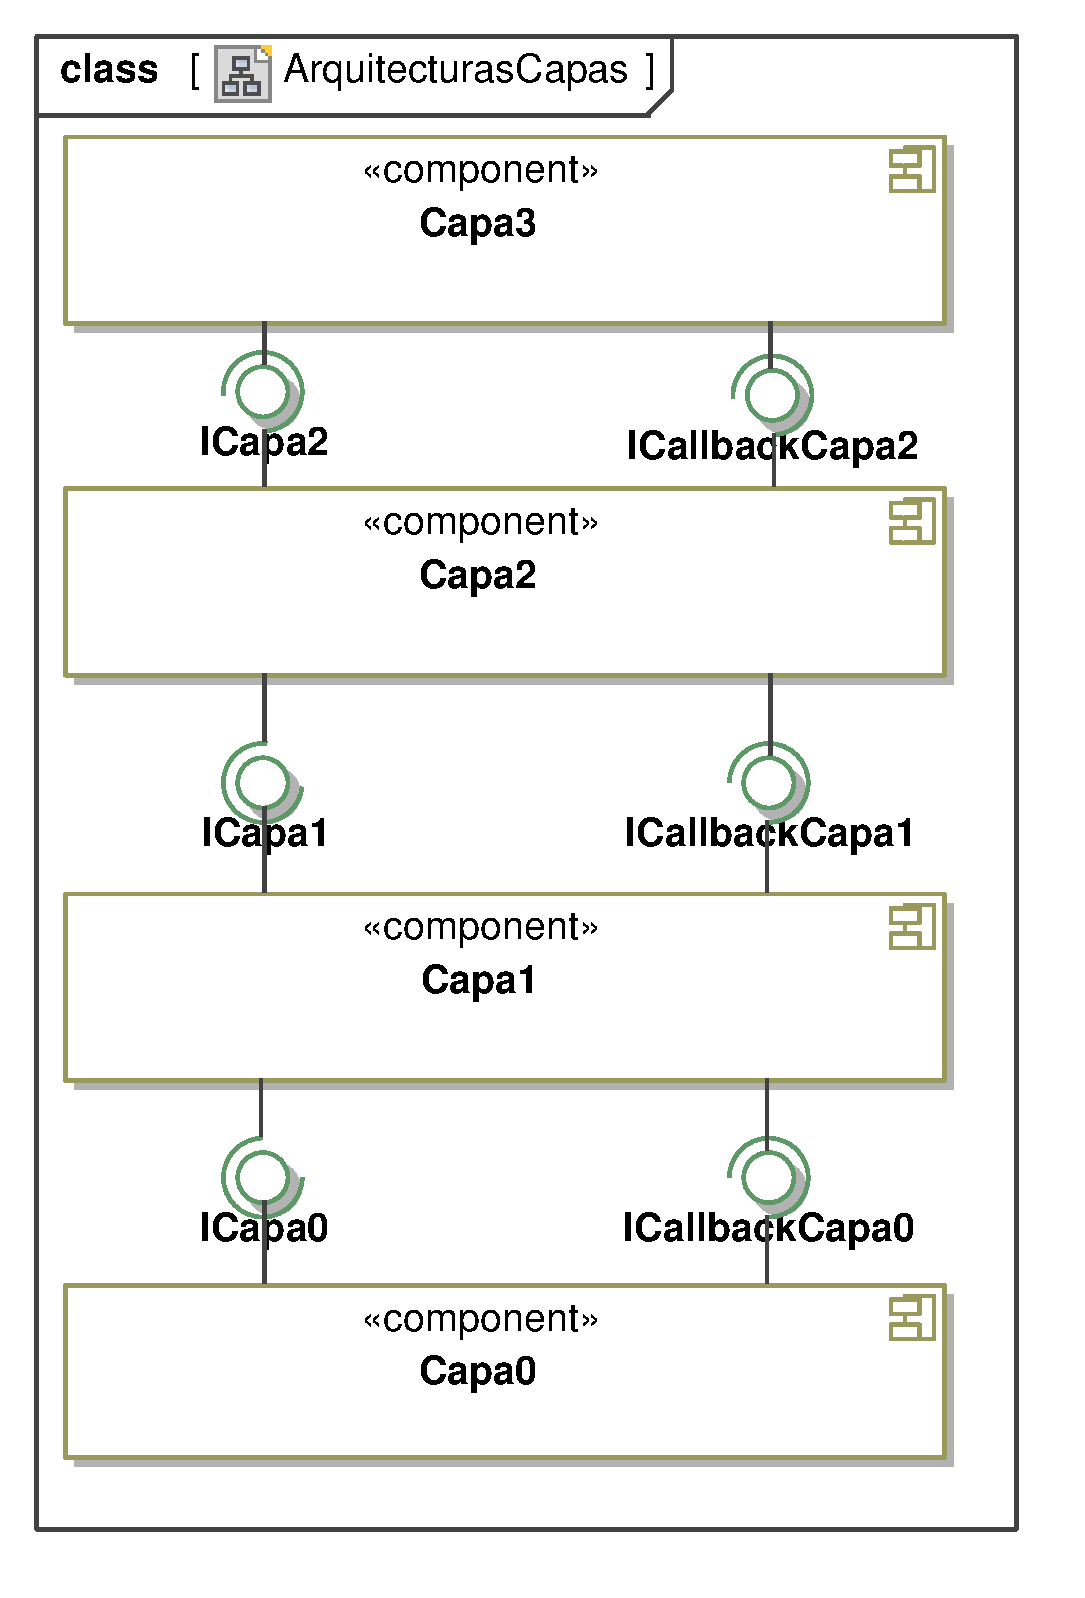
\includegraphics[width=.40\linewidth,keepaspectratio=true]{images/patterns/layered00.eps}
	\end{center}
\end{frame}

\begin{frame}[c]
	\frametitle{Arquitecturas en Capas}
	\begin{center}
        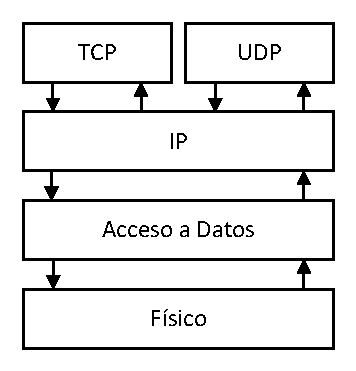
\includegraphics[width=.5\linewidth,keepaspectratio=true]{images/patterns/layered01.eps}
	\end{center}
\end{frame}

\begin{frame}[c]
    \frametitle{Arquitecturas en Capas - Beneficios}
    \begin{enumerate}[<+->]
        \item Permite controlar y gestionar la complejidad de un sistema software.
        \item Independencia y capacidad de reemplazo de las capas.
    \end{enumerate}
\end{frame}

\begin{frame}[c]
    \frametitle{Arquitecturas en Capas - Problemas}
    \begin{enumerate}[<+->]
        \item Rendimientos.
        \item Esfuerzo requerido para el diseño.
        \item Elementos no fácilmente aislables en capas.
    \end{enumerate}
\end{frame}

\subsubsection{Arquitecturas en Cliente-Servidor}

\begin{frame}[c]
    \frametitle{Arquitecturas Cliente/Servidor - Principio Básico}
    \begin{block}{Arquitecturas Cliente/Servidor}
        \begin{itemize}[<+->]
            \item Existe un nodo especializado denominado \emph{servidor}.
            \item El servidor centraliza ciertos cómputos del sistema.
            \item Los clientes realizan peticiones al servidor, el cual las procesa y devuelve las respuesta a los clientes.
        \end{itemize}
    \end{block}
\end{frame}

\begin{frame}[c]
	\frametitle{Arquitecturas Cliente/Servidor}
	\begin{center}
        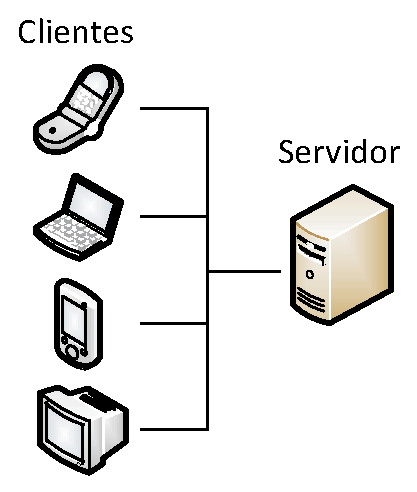
\includegraphics[width=.5\linewidth,keepaspectratio=true]{images/patterns/clienteServidor.eps}
	\end{center}
\end{frame}

\begin{frame}[c]
    \frametitle{Arquitecturas Client/-Servidor - Beneficios}
    \begin{enumerate}[<+->]
        \item Ubicuidad del sistema.
        \item Facilidad de mantenimiento y actualización.
        \item Eliminación de redundancias y posibles inconsistencias.
        \item Permite aligerar los necesidades hardware de los clientes.
        \item Permite trabajar con clientes heterogéneos.
    \end{enumerate}
\end{frame}

\begin{frame}[c]
    \frametitle{Arquitecturas Cliente-Servidor - Problemas}
    \begin{enumerate}[<+->]
        \item Efecto estrella de la muerte.
        \item Disponibilidad del servidor.
        \item Problemas de escalabilidad y rendimiento.
        \item Saturación de las redes de comunicación.
    \end{enumerate}
\end{frame}

\subsubsection{Patrón Código Móvil}

\begin{frame}[c]
    \frametitle{Código Móvil - Principio Básico}
    \begin{block}{Arquitecturas con Código Móvil}
        Un computador (genera y) almacena código y/o datos que se envían a otros computadores para su ejecución.
    \end{block}
\end{frame}

\begin{frame}[c]
    \frametitle{Arquitecturas con Código Móvil - Beneficios}
    \begin{enumerate}[<+->]
        \item Permite distribuir y equilibrar la carga de trabajo.
        \item Permite aumentar la disponibilidad y tolerancia a fallos del sistema.
        \item Facilitar el mantenimiento y la evolución del sistema.
        \item Ubicuidad de ciertas funciones del sistema.
        \item Utilización y composición de recursos bajo demanda.
    \end{enumerate}
\end{frame}

\begin{frame}[c]
    \frametitle{Arquitecturas con Código Móvil - Problemas}
    \begin{enumerate}[<+->]
        \item Agujeros de seguridad.
        \item Saturación de las redes de comunicación.
    \end{enumerate}
\end{frame}

\section{Arquitecturas en Capas de los Sistemas de Información Empresarial}

\begin{frame}[c]
	\frametitle{Capas de un Sistema Empresarial}
	\begin{center}
        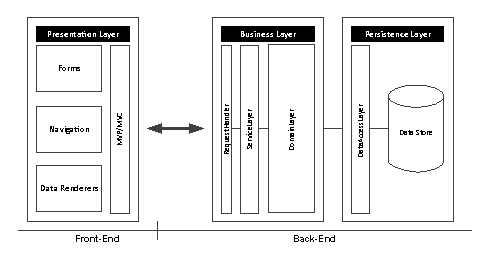
\includegraphics[width=\linewidth,keepaspectratio=true]{images/enterpriseLayers/enterpriseLayers.eps}
	\end{center}
\end{frame}

\begin{frame}[c]
	\frametitle{Responsabilidades de la Capa de Presentación}
	\begin{enumerate}[<+->]
        \item Permitir a los usuarios interactuar con el sistema.
        \item Introducir datos en el sistema (validándolos previamente).
        \item Visualizar los datos de manera amigable al usuario.
        \item Facilitar operaciones simples (filtros y redistribuciones) sobre los datos.
        \item Facilitar la navegación por el sistema.
        \item Mejorar la experiencia de usuario (UX). %% Hellmans
        \item Mantener la comunicación con el servidor.
        \item Gestionar situaciones excepcionales.
	\end{enumerate}
\end{frame}

\begin{frame}[c]
	\frametitle{Responsabilidades de la Capa de Persistencia}
	\begin{enumerate}[<+->]
        \item Almacenar los datos de manera no volátil.
        \item Recuperar datos del almacén persistente,
        \item Asegurar la disponibilidad de los datos.
        \item Controlar la integridad de los datos.
        \item Asegurar un acceso eficiente a los datos.
	\end{enumerate}
\end{frame}

\subsubsection{Capa de Negocio}

\begin{frame}[c]
	\frametitle{Responsabilidades de la Capa de Negocio}
	\begin{enumerate}[<+->]
        \item Asegurar que los datos se manipulan de acuerdo con las \alert{reglas de negocio} existentes.
        \item Asegurar la \alert{transaccionalidad} de las operaciones.
        \item Atender las peticiones de los clientes.
        \item Validar las peticiones de los clientes.
        \item Recuperar y almacenar datos del almacén o almacenes persistentes.
        \item Facilitar la eficiencia del sistema.
        \item Ayudar a mejorar la experiencia de usuario.
        \item Controlar el acceso a los datos.
        \item Gestionar la comunicación con los servicios externos.
        \item Ejecutar operaciones periódicas de mantenimiento.
        \item Gestionar de manera adecuada casos excepcionales.
	\end{enumerate}
\end{frame}

\subsubsection{¿Por qué se utilizan tecnologías Web?}

\begin{frame}[c]
	\frametitle{¿Por Qué Tecnologías Web?}
    \centering \textbf{Ventajas} \\
    \begin{enumerate}
        \item<2-> Multiplataforma.
        \item<3-> Onmipresencia de la web.
        \item<4-> No precisan permisos especiales a nivel de red.
        \item<5-> Patrón código móvil.
        \item<6-> Facilidad de mantenimiento.
        \item<7-> Fuerte estandarización.
        \item<8-> Facilidad de uso.
        \item<9-> Madurez de las herramientas.
    \end{enumerate}
    \uncover<10->{
        \centering \textbf{Inconvenientes} \\
        \begin{enumerate}
        \item Seguridad.
        %% Comentar el problema de los ciberataques rusos y las tostadores americanas.
        %% Añadir a moodle la imagen: http://i.imgur.com/GGiKG9z.jpg
        %% https://goo.gl/ypz4VD
        \item Tecnologías desarrolladas para el intercambio de hipertexto.
        \end{enumerate}
    }
\end{frame}

\subsection{Tecnologías de Implementación para Arquitecturas Empresariales}

\begin{frame}[c]
	\frametitle{Tecnologías de Implementación ES}
	\begin{center}
        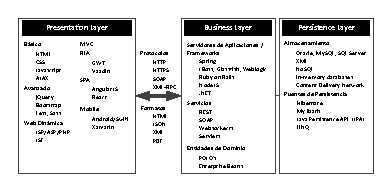
\includegraphics[width=\linewidth,keepaspectratio=true]{images/enterpriseLayers/technologies.eps}
	\end{center}
\end{frame}

\subsection{Distribución de Capas en Arquitecturas Empresariales}

\begin{frame}[c]
	\frametitle{Despliegue de Aplicaciones Empresariales}
	\begin{enumerate}[<+->]
        \item Front-end en el cliente y back-end en uno o más servidores.
        \item Dominio y persistencia pueden ir en el mismo servidor (\emph{two tier}) o en servidores separados (three tiers).
        \item Trabajo con conexión puede requerir parte de la capa de dominio (y persistencia) en el cliente.
        \item Los clientes pueden ser pesados (PCs) o ligeros (Smartphones, tablets).
        \item La capa de presentación puede ser de código fijo (app, desktop) o móvil (HTML + Javascript).
	\end{enumerate}
\end{frame}

\section{Inyección de Dependencias}

\section{Sumario y Referencias}

\begin{frame}[c]
    \frametitle{¿Qué Tengo que Saber de Todo Esto?}
    \begin{enumerate}[<+->]
        \item TODO
    \end{enumerate}
\end{frame}

\subsection{Referencias}

\begin{frame}
	\frametitle{Referencias}
    \nocite{}
	\bibliographystyle{apalike}
    \bibliography{arqEmp}
\end{frame}

\end{document}
